\section{Verteilte Anwendungen mit RMI}\label{sec:distributedrmiapplications}

\begin{tcolorbox}
\blockquote[{\url{https://docs.oracle.com/en/java/javase/21/docs/specs/rmi/intro.html} - abgerufen 22.2.2024}]{
    The Java platform's remote method invocation system [...] has been specifically designed to operate in the Java application environment. The Java programming language's RMI system assumes the homogeneous environment of the Java virtual machine (JVM), and the system can therefore take advantage of the Java platform's object model whenever possible.
}
\end{tcolorbox}

Wenn man eine verteilte Java-Anwendung entwickeln soll, bei der Kommunikationsprotokoll und Client- und Server-Seite in Java implementiert werden, ist \textbf{RMI} die bessere Alternative gegenüber  \textbf{Sockets} (vgl.~\cite[311]{Oec22}).

\begin{tcolorbox}[enlarge top by=0.5cm,enlarge bottom by=0.5cm]
    \textbf{Remote Method Invocation} ermöglicht das Aufrufen von Methoden auf Objekten, die sich auf demselben oder einem anderem Rechner als der Aufrufer befinden, und damit als unterschiedliche Prozesse in unterschiedlichen Adressräumen ausgeführt werden.
\end{tcolorbox}

\noindent
\textbf{Remote Method Invocation} (RMI) stellt eine Schnittstelle zur Nutzung der Internetprotokolle \textbf{TCP} und \textbf{UDP} bereit.\\
Für RMI ist ein Protokoll auf Schicht 5 definiert.
Das Protokoll legt Reihenfolge und Codierung für Daten bei Methodenaufrufen und Methodenrückkehr fest (vgl.\cite[402]{Oec22}).

\noindent
\textbf{RMI} verfolgt den Ansatz, OOP auch für die Kommunikation zwischen verteilten Anwendungen zu realisieren, wobei der Aspekt der Verteilung für die Entwickler weitestgehend transparent bleibt


\noindent
Die \textbf{Verteilungstransparenz} wird bei \textbf{RMI} über \textbf{Stubs} und \textbf{Skeletons} realisiert.\\

\noindent
Ein \textbf{Stub} implementiert dieselbe Schnittstelle wie das Objekt, das über Fern-Methodenaufrufe \textit{auf dem Server gesteuert werden soll}.

\noindent
Ein \textbf{Skeleton} nimmt die Nachrichten, die vom \textbf{Stub} über die aufgebaute \textbf{TCP}-Verbindung gesendet werden, entgegen und ruft die Methoden auf dem entsprechenden Server-Objekt auf.\\
$\rightarrow$ Ein \textbf{Skeleton} besitzt die Struktur eines \textbf{TCP}-Servers.



\begin{tcolorbox}[enlarge top by=0.5cm,enlarge bottom by=0.5cm]
    Struktur einer RMI Anwendung\footnote{vergleiche zu den folgenden Aussagen~\cite[162 ff.]{HM05}; \textbf{Stubs} und \textbf{Skeletons} werden automatisch generiert.}:\\


    \noindent
    \textbf{RMI-Client}\\
    Ein \textbf{RMI-Client} fragt bei einem \textbf{RMI-Namensdienst} eine Referenz auf ein entferntes Objekt an, das danach wie ein lokales Objekt behandelt wird.
    Die notwendige Netzwerk-Kommunikation für diese Methodenaufrufe ist transparent und wird automatisch abgewickelt.\\


    \noindent
    \textbf{Stub-Objekt}
    \begin{itemize}
        \item Ein \textbf{Stub-Objekt} ist ein \textbf{Stellvertreter} für das entfernte Objekt bei dem RMI-Server.
        Methodenaufrufe des \textbf{RMI-Clients} auf ein entferntes Objekt werden an das Stub-Objekt \textit{delegiert}.
        \item Verantwortlichkeiten: Weiterleitung von Methodenaufrufe an das entfernte Objekt. \textit{Marshalling} von Übergabeparametern und \textit{unmarshalling} von Rückgabewerten\footnote{
          Serialisierung: Umwandeln einer Objektstruktur in ein speicherbares Format. Marshalling bezieht sich auf das Bewegen von Objekten zwischen Threads und Programmen, wofür auch eine Form von Serialisierung notwendig ist. S. a. ``Marshalling (computer science): \url{https://en.wikipedia.org/wiki/Marshalling_(computer_science)} - abgerufen 1.2.2024
        }.
        \item Der Stub wird für jede Anwendung automatisch erzeugt (vgl.\cite[313]{Oec22}).
    \end{itemize}\\

    \noindent
    \textbf{Skeleton-Objekt}\\
   Ein \textbf{Skeleton-Objekt} ist ein \textit{server-seitiger} \textbf{Stellvertreter} für das aufrufende Objekt bei dem RMI-Server, und unterstützt ebenfalls  \textit{Marshalling} von Übergabeparametern und \textit{unmarshalling} von Rückgabewerten.
    Das Skeleton-Objekt ist als Programmteil in der RMI-Implementierung dabei und kann für alle RMI-Anwendungen verwendet werden (vgl.\cite[313]{Oec22}).\\

    \noindent
    \textbf{RMI-Registry}\\
    Die \textbf{RMI-Registry} realisiert einen \textit{Namensdienst}: Eine Abbildung von Namen auf entfernte Objekte.\footnote{
        s.a: ``Kapitel 6: Verteilte Objekte durch RMI``: \url{https://www.informatik.uni-marburg.de/~mathes/download/k6.pdf}, ``Distributed object communication``: \url{https://en.wikipedia.org/wiki/Distributed_object_communication} - beides abgerufen 1.2.2024
    }. \\
    Der \textbf{RMI-Client} fordert hier die Referenzen auf entfernte Objekte an.\\

    \noindent
    \textbf{RMI-Server}\\
    Ein \textbf{RMI-Server} instanziiert ein entferntes Objekt und registriert es unter einem Namen bei der \textbf{RMI-Registry}, und wartet \textit{passiv} auf den Aufruf einer Methode durch den \textbf{RMI-Client}.

\end{tcolorbox}


\begin{figure}
    \centering
    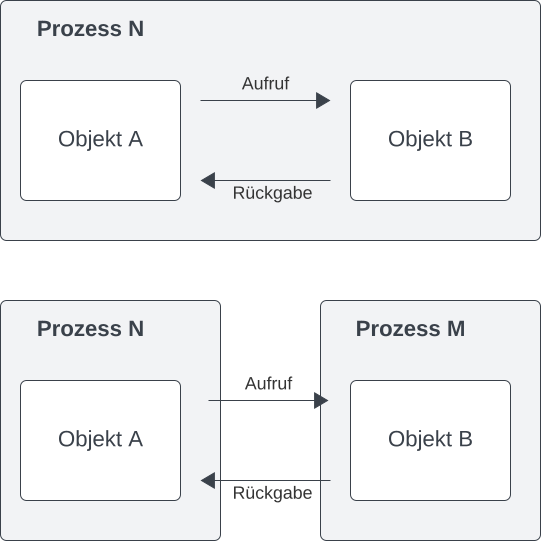
\includegraphics[scale=0.5]{chapters/fopt5/img/rmi/processcall}
    \caption{Zwei unterschiedliche Objekte in unterschiedlichen Aufrufsituationen. Im oberen Beispiel befinden sich die Objekte im selben Adressraum, im unteren Beispiel in unterschiedlichen Adressräumen - diese Situation kommt bei der Nutzung von RMI vor (Quelle: in Anlehnung an \cite[311 f., Abbildung 6.1 und 6.2]{Oec22})}
    \label{fig:processcall}
\end{figure}

\begin{figure}
    \centering
    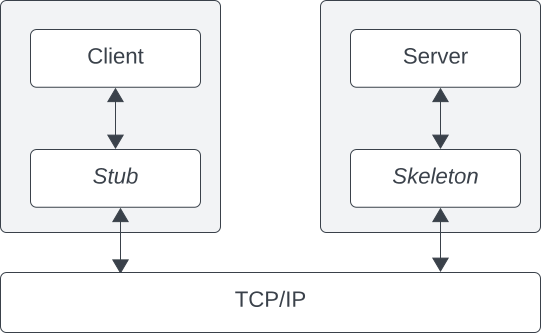
\includegraphics[scale=0.4]{chapters/fopt5/img/rmi/stubskeleton}
    \caption{Prinzip der Kommunikation zwischen RMI-Client und -Server. (Quelle: in Anlehnung an \cite[312, Bild 6.3]{Oec22})}
    \label{fig:stubskeleton}
\end{figure}


\begin{figure}
    \centering
    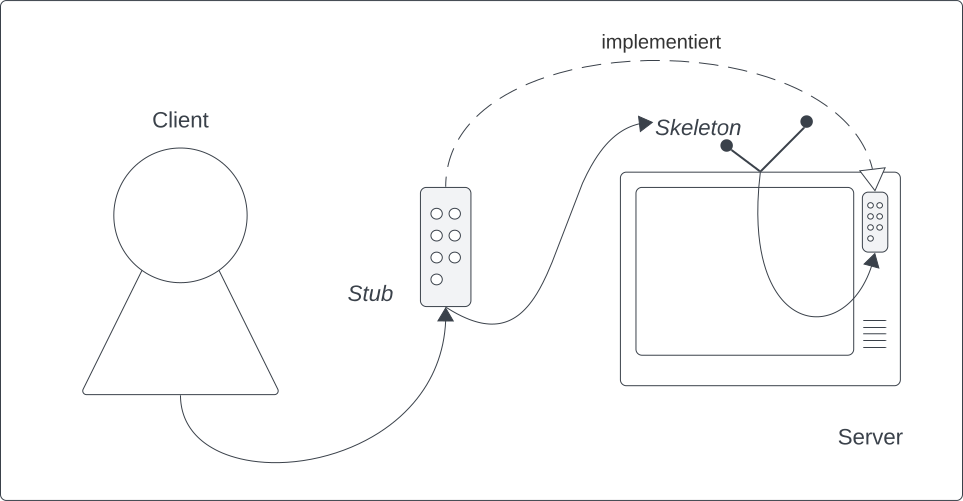
\includegraphics[scale=0.35]{chapters/fopt5/img/rmi/tv}
    \caption{Eine Illustration der im Lehrbuch verwendeten RMI-Metapher. Ein Client will ein entferntes Objekt (TV) bedienen. Hierzu verwendet er Methodenaufrufe, die vom Stub (Fernbedienung) weitergeleitet werden. Die Methoden werden vom Skeleton (Fensehantennen) an das Objekt auf dem Server weitergeleitet. Dieses Objekt sind in dem Beispiel die Knöpfe an dem Fernseher, die die gleichen Bedienfunktionen (``Schnittstelle``) wie die Fernbedienung haben. (Quelle: eigene)}
    \label{fig:tv}
\end{figure}

\noindent
Die \textbf{Transparenz} kommt für den Entwickler dadurch zustande, dass er nur Client und Server, nicht aber Stub und Skeleton programmieren muss.\\
$\rightarrow$ \textbf{Stub} wird automatisch erzeugt, das \texbf{Skeleton}-Objekt ist ein Programmteil, der in der \textbf{RMI}-Implementierung dabei ist und für alle Anwendungen verwendet werden kann.\\

\noindent
Die Entwicklung einer \textbf{RMI}-Anwendung erfolgt i.d.R. in folgenden Schritten\footnote{
s.a. ``An Overview of RMI Applications``: \url{https://docs.oracle.com/javase/tutorial/rmi/overview.html} - abgerufen 1.2.2024
}:

\begin{enumerate}
    \item\label{itm:intdef} \textbf{Schnittstelle definieren}\\
    \noindent
    Die Schnittstelle zwischen Client \& Server in Abhängigkeit von der Anwendung, die realisiert werden soll.\\
    \noindent
    Die Schnittstelle führt alle Methoden auf, die über \textbf{RMI} aufgerufen werden sollen.\\
    \noindent
    Die Schnittstelle muss aus \code{java.rmi.Remote} abgeleitet werden.\\
    \noindent
    Alle Methoden der Schnittstelle müssen mit \code{throws RemoteException} gekennzeichnet werden\footnote{
    s.a. ``2.4.1 The java.rmi.Remote Interface``: \url{https://docs.oracle.com/en/java/javase/21/docs/specs/rmi/objmodel.html#the-java.rmi.remote-interface} - abgerufen 1.2.2024
    }.

    \item \textbf{Schnittstelle implementieren}\\
    \noindent
    Es wird eine Klasse geschrieben, die die im ersten Schritt definierte Schnittstelle implementiert.\\
    \noindent
    Ein Objekt davon muss \textit{von außen über RMI} nutzbar sein - es muss exportiert werden können.
    Dazu kann die implementierende Klasse von \code{UnicastRemoteObject} abgeleitet werden.\\
    Es muss ein expliziter Konstruktor existieren, der mit \code{throws RemoteException} gekennzeichnet wird. \\
    $\rightarrow$ Es muss mindestens ein expliziter Standard-Konstruktor existieren, der diese Bedingung erfüllt\footnote{
    ansonsten wird vom Compiler ein Standard-Konstruktor zur Verfügung gestellt.
    Da dieser aber keine checked Exception in Form einer \textit{RemoteException} wirft, kommt es zu einem Compilerfehler.
    }

    \item \textbf{Server programmieren}\\
    \noindent
    Man erzeugt eines oder mehrere Objekte der in Schritt 2 implementierten Klasse und meldet diese unter einem beliebigen Namen bei der \textbf{RMI-Registry} an.

    \item \textbf{Client programmieren}\\
    \noindent
    Über die \textbf{RMI-Registry} (Serveradresse und Port müssen dem Client bekannt sein) beschafft sich der Client die in Schritt 3 registrieren Objekte, die als \textbf{Stub} an ihn weitergeleitet werden.\\
    \noindent
    Der Stub kann unter Berücksichtigung der in Schritt 1 definierten Schnittstelle so verwendet werden, als wäre es ein lokales Objekt\footnote{
    ``lokal`` im Sinne von gleicher Prozess / gleicher Adressraum.
    }.\\
    \noindent
    Die Methodenaufrufe werden dann letztendlich auf dem durch das in Schritt 2 definierte \textbf{RMI-Objekt} auf dem Server ausgeführt (Client $\rightarrow$ Stub $\rightarrow$ Skeleton $\rightarrow$ Server).

    \item \textbf{Anwendung übersetzen und ausführen}\\
    \noindent
    Alle Dateien werden kompiliert.
    Vor dem Starten des Programms ist darauf zu achten, dass auf dem Server die \textbf{RMI-Registry} gestartet wird - was aber auch aus dem Programm heraus geschehen kann.
\end{enumerate}

\subsection{Einführendes RMI-Beispiel}\label{sec:rmiintro}

Auch bei RMI-Implementierungen bei denen mehrere Clients gleichzeitig auf eine Objektinstanz zugreifen, ist (ggf. nach Anwendung) \code{synchronized} nötig, um ein Objekt für den gleichzeitigen Zugriff zu sperren.\\

\noindent
Sobald über \staticcode{java.rmi.Naming.rebind()} bzw. \staticcode{bind()}\footnote{
\textit{bind()} wirft eine \textit{AlreadyBoundException}, falls in der RMI-Registry bereits ein Eintrag mit dem Namen existiert, \textit{rebind()} hingegen ersetzt einen ggf. breits existierenden Eintrag mit gleichem Namen.
} der Server gestartet wurde, wird ein Thread gestartet, der den Skeleton repräsentiert, und auf eingehende TCP-Verbindungen wartet.\\

\noindent
Der Client fragt vom Server über

\begin{minted}[mathescape,
    numbersep=5pt,
    gobble=2,
    frame=none,
    framesep=2mm]{java}
    java.rmi.Naming.lookup("rmi://serveradresse/bindingname");
\end{minted}\\

\noindent
das Objekt ab, auf das er zugreifen möchte, und bekommt dann ein Objekt vom Typ \code{java.rmi.Remote} zurück.\\
Das Objekt muss noch zu dem Typen gecasted werden, der in ``Schnittstelle definieren`` in Punkt~\ref{itm:intdef} (s. vorheriger Abschnitt) implementiert wurde, um entsprechende Methoden der implementierten Schnittstelle aufrufen zu können (das über \code{lookup()} zurückgegebene Objekt ist das \textbf{Stub-Objekt}).\\

\noindent
Bevor der Server auf dem entsprechenden Rechner gestartet wird, muss auf diesem Rechner über die Konsole noch \code{rmiregistry} aufgerufen werden, damit die \textbf{Registry} zur Verfügung steht, sofern das nicht wie im folgenden Beispiel über das Programm geschieht.
Das Listing zeigt die Implementierung für einen einfachen Echo-Server\footnote{
``Echo Protocol``: \url{https://en.wikipedia.org/wiki/Echo_Protocol} - abgerufen 2.2.2024
}.\\
Die RMI-Registry wird hierbei ebenfalls über das Programm gestartet.
\begin{minted}[mathescape,
linenos,
numbersep=5pt,
gobble=2,
fontsize=\small,
frame=lines,
framesep=2mm]{java}
    public class RMIDemo {

        interface Echo extends Remote {
            String echo(String msg) throws RemoteException;
        }

        static class EchoImpl extends UnicastRemoteObject implements Echo {

            public EchoImpl() throws RemoteException{}

            @Override
            public String echo(String msg) throws RemoteException {
                return msg;
            }
        }

        public static void main(String[] args) {
            if (args.length == 0) { // Server
                try {
                    Registry registry = LocateRegistry.createRegistry(1099);
                    registry.rebind("echo", new EchoImpl());
                } catch (RemoteException e) {
                    System.err.println("[registry] " + e);
                }
                return; //Thread is started, it's okay to leave main() at this point.
            }
            // client
            try {
                Remote stub = Naming.lookup("rmi://localhost:1099/echo");
                Echo echo = (Echo) stub;
                System.out.println(echo.echo(args[0]));
            } catch (NotBoundException | MalformedURLException | RemoteException e) {
                System.err.println("[client] " + e);
            }
        }
    }
\end{minted}

\begin{tcolorbox}[enlarge top by=0.5cm,enlarge bottom by=0.5cm]
    RMI-Methodenaufrufe sind blocking, auch wenn der Rückgabetyp für die aufgerufene Methoden mit \code{void}-deklariert wurde.\\

    \blockquote[{``3.1 Stubs and Skeletons``: \url{https://docs.oracle.com/en/java/javase/21/docs/specs/rmi/arch.html} - abgerufen 2.2.2024 (Hervorherbungen eigene)}]{
        When a stub's method is invoked, it does the following:
        \begin{itemize}
            \item initiates a connection with the remote JVM containing the remote object,
            \item marshals (writes and transmits) the parameters to the remote JVM,
            \item \textbf{waits for the result of the method invocation},
            \item \textbf{unmarshals (reads) the return value or exception returned}, and
            \item returns the value to the caller.
        \end{itemize}

    }
\end{tcolorbox}

\subsection{RMI-Client mit grafischer Benutzeroberfläche}

In Listing 6.5 (\cite[320]{Oec22}) wird bei jedem Buttonclick ein neuer Thread gestartet.
Die gestarteten Threads können unterschiedlich schnell ablaufen, und somit zu unerwarteten Ergebnissen führen:

\blockquote[{\cite[323]{Oec22}}]{
[...] man wird vermutlich davon ausgehen, dass der angezeigte Zählerwert immer derjenige ist, der aus der eigenen zuletzt angestoßenen Aktion resultiert.
    Aber dies muss nicht in jedem Fall so sein.
}

Als Lösung könnte man die ankommenden Aufträge durch einen einzigen Thread ausführen lassen, indem die Aktionen {bspw.} in eine Warteschlange eingereiht werden (vgl.~\cite[323]{Oec22}).

\newpage
In dem o.a. Listing wird das Functional Interface \code{Consumer}\footnote{
`´Interface Consumer<T>``: \url{https://docs.oracle.com/en/java/javase/21/docs/api/java.base/java/util/function/Consumer.html} - abgerufen 2.2.2024
} verwendet.
Folgendes Beispiel stellt die Verwendung in vereinfachter Form nochmal dar:


\begin{minted}[mathescape,
    linenos,
    numbersep=5pt,
    gobble=2,
    fontsize=\small,
    frame=lines,
    framesep=2mm]{java}
    public class ConsumerDemo {
        interface Supplier<T> {
            T execute();
        }

        public <T> void asyncCall(Supplier<T> s, Consumer<T> c) {
            startThread(s, c);
        }

        public <T> void startThread(Supplier<T> s, Consumer<T> c) {
            Thread t = new Thread(() -> c.accept(s.execute()));
            t.start();
        }

        public static void main(String[] args) {
            ConsumerDemo cd = new ConsumerDemo();
            cd.asyncCall(
                () -> Math.random() * 100,
                (r) -> System.out.println("Done: " + r)
            );
        }
    }
\end{minted}\\

\begin{tcolorbox}
    Generell ist zu berücksichtigen, dass RMI-Aufrufe blocking sind.\\
    Wird also aus einem Programm heraus ein RMI-Methodenaufruf durchgeführt, und ist eine grafische Benutzeroberfläche abhängig von den Rückgabewerten, sollte der Aufruf in einem Thread sttatfinden.\\
    Die Antwort des RMI-Methodenaufrufes sollten dann über \code{Runnable}s and \code{Platform.runLater()} übergeben werden - der Übergabeparameter landet bekanntlich in einer event queue, deren Einträge dann zu einem in der Zukunft liegenden unbestimmten Zeitpunkt auf dem \textbf{JavaFX Application Thread} aufgerufen werden.\\
    Werden gleichzeitig mehrere Methoden ein und desselben RMI-Objektes von unterschiedlichen Clients aufgerufen, sollten die Methoden \code{synchronized} sein, falls es die Implementierung des passiven Objektes erfordert.
\end{tcolorbox}

\subsection{RMI-Registry}

\code{java.rmi.Naming} stellt die Methode \staticcode{bind()} zur Verfügung - wenn die Methode aufgerufen wird, und der Name schon vergeben (``gebunden``) ist, wird eine \code{AlreadyBoundException} geworfen; für ein \textit{rebinding} müsste die \textbf{RMI-Registry} neugestartet werden; aus dem Grund kann man \staticcode{rebind()} verwenden.\\
Wenn ein Server herunterfährt, sollte man auch mittels \staticcode{unbind()} die von ihm vorher registrierten RMI-Objekte wieder abmelden.

\begin{tcolorbox}[enlarge top by=0.5cm,enlarge bottom by=0.5cm]
    \code{bind()}, \code{rebind()} und \code{unbind()}, ruft der Server auf, der sich auf dem gleichen Rechner befinden muss wie die \textbf{Registry}.\\
    \noindent
    \code{lookup()} und \code{list()} ruft i.d.R. der Client auf, der auf einem beliebigen Rechner laufen kann.
\end{tcolorbox}

\noindent
Eine weitere statische Methode ist \staticcode{list():String[]}, die einem ein Feld mit allen Einträgen der Registry zurückliefert.\\

\noindent
Die Kommunikation zwischen \textit{Client und Server}, \textit{Client und Registry} sowie \textit{Server und Registry} findet über \textbf{TCP-Sockets} statt.\\

\noindent
Die \textbf{Registry} startet standardmäßig auf Port $1099$.\\

\noindent
Ein Server startet auf einer beliebigen freien Portnummer; während der Registrierung werden einem Objekt weitere Informationen zugeordnet, wie Portnummer und eine \textit{Objekt-Id-Kennung}, damit man das Objekt erreichen kann.\\
Wenn der Client mittels \staticcode{java.rmi.Naming.lookup(name:String)} einen Eintrag aus der Registry anfordert, enthält das zurückgegebene Objekt diese Informationen.
Diese Informationen können dann zur Verbindungsherstellung genutzt werden.

\begin{tcolorbox}[enlarge top by=0.5cm,enlarge bottom by=0.5cm]
    Ein Server kann mehrere Objekte beherbergen, die alle unter ein und derselben Portnummer erreichbar sind (vgl.~\cite[324]{Oec22}).
\end{tcolorbox}

\begin{figure}
    \centering
    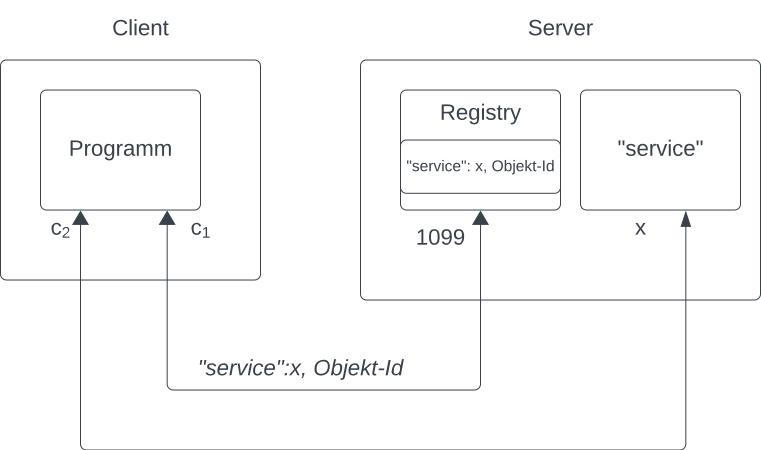
\includegraphics[scale=0.5]{chapters/fopt5/img/rmi/registry}
    \caption{Ein Client fragt den Eintrag der Registry für ``service`` ab und erhält über den Port des Client-Rechners $c_1$ die Erreichbarkeitsinformationen, die u.a. aus einer Portnummer $x$ und einer Objekt-Kennung bestehen.
    Antworten auf seine Anfragen werden daraufhin an seinen Port $c_2$ gesendet. (Quelle: in Anlehnung an \cite[324, Bild 6.5]{Oec22})}
    \label{fig:registry}
\end{figure}

Die \textbf{Registry} lässt sich auch aus dem Programm heraus starten\footnote{
``Class LocateRegistry``: \url{https://docs.oracle.com/en/java/javase/21/docs/api/java.rmi/java/rmi/registry/LocateRegistry.html} - abgerufen 2.2.2024
}:

\begin{minted}[mathescape,
    numbersep=5pt,
    gobble=2,
    frame=none,
    framesep=2mm]{java}
    java.rmi.registry.LocateRegistry.createRegistry(port:int):Registry
\end{minted}\\

\noindent
Der zurückgegebene Typ implementiert \code{java.rmi.registry.Registry} und besitzt dieselben Methoden wie \code{java.rmi.Naming}\footnote{was aber nicht heißt, dass \textit{Naming} auch \textit{Registry} implementiert - die Methoden von \textit{Naming} sind allesamt statisch.
}.\\
$\rightarrow$ Entweder wird die Registry nur in einem Server gestartet, oder weitere Registries müssen eigene, unterschiedliche Portnummern enthalten.

\subsection*{Eigene Notizen}

Länger andauernde Aufträge an ein Remote-Objekt sollten über Threads realisiert werden.\\

\noindent
Muss eine UI während / infolgedessen aktualisiert werden, sollte diese UI-Aktualisierung über \code{javafx.application.Platform.runLater()} stattfinden (\textbf{JavaFX Application Thread}).


\subsection{Parallelität bei RMI-Methodenaufrufen}\label{sec:rmiparallel}


\begin{tcolorbox}
Ein \textbf{Skeleton} ist ein paralleler \textbf{TCP-Server} (vgl.\cite[329]{, Oec22}).
\end{tcolorbox}

\begin{tcolorbox}[enlarge top by=0.5cm,enlarge bottom by=0.5cm]
    Identität und Gleichheit von zwei \textbf{Stubs}:\\
    \noindent
    Rückgabewert von \code{Naming.lookup(...)} führt bei Objektvergleich mittels $==$zu \code{false}, wenn ein Stub für ein und denselben Namen zweimal angefordert wird, \code{equals()} hingegen zu \code{true}.\\

    $\rightarrow$ \textbf{Stub-Objekte} sind in diesem Fall nicht ``identisch``, aber wenn sie auf dasselbe \textbf{RMI-Objekt} zeigen, werden sie als ``gleich`` betrachtet.\\

    ``Zwei Stub-Objekte sind genau dann gleich, wenn sie eine Referenz auf dasselbe Objekt in der Ferne repräsentieren.`` (\cite[347]{Oec22})
\end{tcolorbox}\\

\noindent
Wird ein \textbf{Stub} angefordert, der eine asynchrone Operation ausführt, und dieser Stub wird in einen Thread ausgelagert, verhält sich der Stub \textit{intelligent}:

\begin{itemize}
    \item \textit{wenn mehrere Threads erzeugt werden}, und ``parallel`` gearbeitet wird, werden die Operationen auch parallel ausgeführt, und zwar indem mehrere Verbindungen aufgebaut werden (dadurch werden auf Server-Seite mehrere Threads erzeugt).
    \item wird auf Client-Seite keine parallele Ausführung durch die Erzeugung von Threads erzwungen, findet die Abarbeitung der Operation(en) sequentiell statt, es wird dann auch nur eine Verbindung dafür aufgebaut.
    \item ein einzelner Stub ist also auch dazu in der Lage, parallele Aufrufe auf dem Server zu erzeugen
\end{itemize}

\begin{tcolorbox}[enlarge top by=0.5cm,enlarge bottom by=0.5cm]
    \cite[330]{Oec22} weist darauf hin, dass Methodenaufrufe auf ein RMI-Objekt parallel stattfinden durch mehrere Clients - beim gleichzeitigen Zugriff auf gemeinsame Daten muss entsprechend synchronisiert werden\footnote{
        s.a. ``3.2 Thread Usage in Remote Method Invocations``: Die Spezifikationen scheinen hier keinen Hinweis darauf zu geben, dass es eine Garantie für die Threads gibt. \url{https://docs.oracle.com/en/java/javase/21/docs/specs/rmi/arch.html#thread-usage-in-remote-method-invocations} - abgerufen 2.2.2024
    }.
\end{tcolorbox}

\begin{tcolorbox}[colback=red!20,color=white,title=Anmerkung]
    Bzgl. \cite[330]{Oec22} geben die Spezifikationen unter ``3.2 Thread Usage in Remote Method Invocations``\footnote{
        \url{https://docs.oracle.com/en/java/javase/21/docs/specs/rmi/arch.html#thread-usage-in-remote-method-invocations} - abgerufen 2.2.2024
    } keinen Hinweis darauf, dass Threads garantiert erzeugt werden.
\end{tcolorbox}

\subsection{Wertübergabe für Parameter und Rückgabewerte}\label{sec:valuermi}

Bei \textbf{RMI} können Objektparameter oder Objektrückgabewerte als \textbf{Wert} oder \textbf{Referenz} übergeben werden.\\

\noindent
Bei der Übergabe als Wert wird eine Kopie des Objektes erzeugt, und zwar rekursiv bei gleichzeitiger Vermeidung von Zyklen.\\

\noindent
Diese Kopie wird dann auf dem Server in der entsprechenden Methode aufgerufen:

\begin{tcolorbox}[enlarge top by=0.5cm,enlarge bottom by=0.5cm]
    Damit ein Objekt auf einen Server übertragen werden kann, muss es \code{java.io.Serializable} implementieren.
\end{tcolorbox}

\begin{itemize}
    \item wird das Objekt auf dem Server geändert, ändert sich nur \textit{dieses} Objekt auf dem Server, nicht aber das auf dem Client.
    \item[] $\rightarrow$ gibt man dann aber das Objekt als \textit{Rückgabewert} an, sind die geänderten Daten in der Kopie des Objektes vorhanden (wegen Serialisierung und Wertübergabe) - Änderungen daran sind dann aber nicht auf dem Server reflektiert
\end{itemize}

Datenstrukturen werden unter Verwendung von \code{java.io.Serializable} serialisiert {bzw.} deserialisiert; Objekte, die als ``Foge von Bytes`` serialisiert werden sollen, müssen dabei \code{java.io.Serializable} implementieren  - das gilt auch für die Objekte, die mit dem zu serialisierenden Objekt assoziiert sind (vgl.~\cite[332]{Oec22}).\\

\noindent
Bei \textbf{RMI} findet die Serialisierung automatisch statt; möchte man {bspw.} ein Objekt serialisieren und in eine Datei schreiben, muss man die Logik zum Speichern/Lesen des Objektes selber implementieren\footnote{
auch wenn das Beispiel nicht viel Code enthält, sollte klar sein, dass das (De)Serialisieren bei RMI automatisch geschieht und bei Abfrage des Rückgabewerts/ Übergabeparameters bereits erfolgt ist, ohne dass zusätzliche Methoden aufgerufen werden müssen.
}, wie folgendes Beispiel zeigt:\\

\begin{minted}[mathescape,
    numbersep=5pt,
    gobble=2,
    frame=none,
    framesep=2mm]{java}

    // schreiben
    FileOutputStream fos = new FileOutputStream(fileName);
    ObjectOutputStream output = new ObjectOutputStream(fos);
    // hier findet das serialisieren statt
    output.writeObject(obj);
    output.flush();

    //lesen
    FileInputStream fis = new FileInputStream(fileName);
    ObjectInputStream input = new ObjectInputStream(fis);
    // hier findet das de-serialisieren statt
    ConcreteObject obj = (ConcreteObject)input.readObject();
\end{minted}\\

\noindent
Im Wesentliche wird bei der Serialisierung der Zustand eines Objektes gespeichert, was vor allem durch die aktuellen Werte der Attribute des Objektes beschrieben wird.\\

\noindent
Attribute, die bei der Serialisierung nicht berücksichtigt werden sollen, können durch den Feld-Modifier \code{transient} entsprechend gekennzeichnet werden\footnote{
vgl. ``8.3.1.3. transient Fields`` \url{https://docs.oracle.com/javase/specs/jls/se21/html/jls-8.html#jls-8.3.1.3} - abgerufen 2.2.2024
}.


\begin{tcolorbox}[enlarge top by=0.5cm,enlarge bottom by=0.5cm]
    Ein Objekt wird als Wert übergeben, wenn es serialisierbar ist und nicht exportiert ist.
\end{tcolorbox}


\subsection{Referenzübergabe für Parameter und Rückgabewerte}\label{sec:refrmi}

Bei \textbf{RMI} werden Parameter und Rückgabewerte entweder als Wert oder als Referenz übergeben.\\

\noindent
Als \textbf{Wert}, falls eine Klasse \textit{nur} \code{Serializable} implementiert und \textit{nicht} exportiert ist, ansonsten hat die \textbf{Referenzübergabe} Vorrang (bspw. weil die Klasse des Objektes ein Remote Interface ist und von \code{UnicastRemoteObject} abgeleitet ist).

\begin{tcolorbox}[enlarge top by=0.5cm,enlarge bottom by=0.5cm]
    RMI-Objekte implementieren die \code{Remote}-Schnittstelle und sind exportiert, bspw. indem sie von \code{UnicastRemoteObject} abgeleitet sind.\\

    \blockquote[{``5.3.1 Constructing a New Remote Object``: \url{https://docs.oracle.com/en/java/javase/21/docs/specs/rmi/server.html#the-remoteobject-class} - abgerufen 22.2.2024}]{
        A remote object implementation (one that implements one or more remote interfaces) must be created and exported.
    }
\end{tcolorbox}\\

\noindent
Für ein Objekt, das bei \textbf{RMI} als Referenz übergeben wird, wird ein \textbf{Stub} erzeugt, hierzu muss aber nicht extra das betreffende Objekt in einer Registry registriert sein - der Server erhält das \code{Stub}-Objekt nicht über die Registry!\\

\noindent
Eine Übergabe als Referenz ist bspw. dann sinnvoll/ notwendig, wenn der Server auf dem Client Daten ändern muss\footnote{als Beispiel die in Abschnitt 6.5 des Buches vorgestellte Chat-Anwendung - der Server ruft die \textbf{print}-Methode der Clients auf, Clients aktualisieren daraufhin ihr UI mit dem Übergabeparameter... (vgl.~\cite[Listing 6.22, Listing 6.24]{Oec22})}.\\

\noindent
Damit eine Übergabe als Referenz funktioniert, muss das übergebende Objekt vom Typ \code{Remote} (und exportiert) sein.\\

\noindent
Werden \code{UnicastRemoteObjekte} genutzt, erstellen diese zur \textbf{TCP}-Kommunikation Threads.
Deshalb sollte darauf geachtet werden, dass diese Threads beendet sind, bspw. durch einen Aufruf von \code{System.exit(0)}, wenn es zu einem ``kontrollierten`` Programmende kommt\footnote{s. \cite[352]{Oec22}; außerdem ``Shutdown Sequence``: \url{https://docs.oracle.com/en/java/javase/21/docs/api/java.base/java/lang/Runtime.html#shutdown} - abgerufen 2.2.2024
}.

\begin{tcolorbox}[enlarge top by=0.5cm,enlarge bottom by=0.5cm]
    \item Ein Objekt, das eine \textbf{RMI}-Schnittstelle implementiert und von \code{UnicastRemotObject} abgeleitet ist und \textbf{serialisierbar} ist, wird trotzdem als \textbf{Referenz} übergeben.\\

    \noindent
    \textbf{Referenzübergabe} hat Vorrang vor \textbf{Wertübergabe}.\\

    \blockquote[{``5.3.3 Passing a UnicastRemoteObject in an RMI Call``: \url{https://docs.oracle.com/en/java/javase/21/docs/specs/rmi/server.html#the-unicastremoteobject-class} - abgerufen 22.2.2024}]{
        [...] when an exported object of type UnicastRemoteObject is passed as a parameter or return value in an RMI call, the object is replaced by the remote object's stub. An exported remote object implementation remains in the virtual machine in which it was created and does not move (even by value) from that virtual machine. In other words, an exported remote object is passed by reference in an RMI call; exported remote object implementations cannot be passed by value.
    }


\end{tcolorbox}


\subsection*{Spezifikationen}

Die RMI-Spezifikationen\footnote{
\url{https://docs.oracle.com/en/java/javase/21/docs/specs/rmi/index.html} - abgerufen 17.2.2024
} führen unter ``2.6 Parameter Passing in Remote Method Invocation`` die Bedingungen für Wert-/Referenzübergabe auf.\\
Parameter für die Kommunikation bei RMI-Aufrufen können einfache Datentypen (\code{int},  \code{bool},\ldots), serialisierbare Typen (\code{implements} \code{Serializable}) oder exportierte Objekte vom Typ \code{Remote} sein.\\
Unter ``2.6.5 Parameter Transmission`` ist dokumentiert, dass Parameter eines RMI-Aufrufs über ein Objekt vom Typ \begin{center}\code{java.io.ObjectOutputStream}\end{center} in den Output-Stream geschrieben werden.\\
Von besonderem Interesse ist hier die Methode \code{replaceObject(obj: Object): Object}\footnote{
   ``replaceObject``: \url{https://docs.oracle.com/en/java/javase/21/docs/api/java.base/java/io/ObjectOutputStream.html#replaceObject(java.lang.Object)} - abgerufen 17.2.2024
}, deren Verhalten im gleichen Abschnitt wie folgt beschrieben ist:

\blockquote[{(``2.6.5 Parameter Transmission``, ebenda)}]{
    \begin{itemize}
        \item  If the object passed to replaceObject is an instance of java.rmi.Remote and that object is exported to the RMI runtime, then it returns the stub for the remote object. If the object is an instance of java.rmi.Remote and the object is not exported to the RMI runtime, then replaceObject returns the object itself. A stub for a remote object is obtained via a call to the method java.rmi.server.RemoteObject.toStub.
    \item If the object passed to replaceObject is not an instance of java.rmi.Remote, then the object is simply returned.
    \end{itemize}
}




\subsection*{Eigene Notizen}

\noindent
Eine \code{ArrayList} nutzt in ihren Methoden bei Objekten \code{equals} zum Vergleich der enthaltenen Elemente\footnote{
    s. \url{https://docs.oracle.com/en/java/javase/21/docs/api/java.base/java/util/ArrayList.html#equals(java.lang.Object)} - abgerufen 2.2.2024
}.\\

\noindent
Über einen \code{Iterator} können bedenkenlos Objekte entfernt werden, ohne, dass es zu einer \code{ConcurrentModificationException} kommt\footnote{ein Iterator kennt \textit{remove()}, aber kein \textit{add()}. S. \url{https://docs.oracle.com/en/java/javase/21/docs/api/java.base/java/util/Iterator.html#remove()} - abgerufen 2.2.2024}.\\


\noindent
Chatbeispiel: Dem Abmelden von Clients sollte genug Zeit eingeräumt werden - funktioniert das Abmelden nicht richtig, entfernt der Server die fehlerhaften Clients allerdings ohnehin wegen der abgefangenen Exception - s. \cite[345, Listing 6.22]{Oec22}.


\subsection{Transformation lokaler in verteilte Anwendungen}

Um eine lokale Anwendung in eine RMI-Anwendung zu überführen, wird die \textit{passive Klasse} (s. Abschnitt~\ref{subsec:syncsummary}) als Remote-Interface implementiert und von \code{UnicastRemoteObject} abgeleitet.
Daraufhin können Objekte davon als \textbf{RMI-Objekte} von einem Server in der \textbf{RMI-Registry} registriert werden.\\

\noindent
Der Server wartet dann passiv auf Aufrufe durch die \textbf{RMI-Clients}, also Objekte \textit{aktiver Klassen}, die über \code{Naming.lookup()} Zugriffe auf die vom Server zur Verfügung gestellten \code{RMI-Objekte} erhalten.\\

\noindent
Man muss berücksichtigen, dass bei der Entwicklung von RMI-Anwendungen, die mit Sperren arbeiten, die Sperre nicht auf den Objekten auf dem lokalen Rechner gesetzt werden, sondern auf den entfernten Objekten. \\
Wie in Abschnitt~\ref{sec:rmiintro} festgestellt wurde, sind Methodenaufrufe auf RMI-Objekte \textit{blocking}: Ruft also ein Client-Thread auf einem entfernten Objekt eine Methode auf, die den Aufrufer bspw. in eine Warteschlange einfügt, dann ist der Client ebenso lange blockiert wie das in der Warteschlange befindliche Stellvertreterobjekt\footnote{
zu ``Stellvertreterobjekte`` s.a. \url{https://openbook.rheinwerk-verlag.de/java8/14_003.html#u14.3.3} - abgerufen 5.2.2024
}.\\
Ist nun für die RMI-Kommunikation über \begin{center}\code{sun.rmi.transport.tcp.responseTimeout}\end{center} ein Timeout gesetzt, kann es vorkommen, dass aufgrund länger andauernder Prozesse eine \code{java.rmi.RemoteException} geworfen wird:

\blockquote[{``sun.rmi.transport.tcp.responseTimeout``: \url{https://docs.oracle.com/javase/8/docs/technotes/guides/rmi/sunrmiproperties.html} - abgerufen 5.2.2024, Hervorhebungen entfernt}]{
    The value of this property represents the length of time (in milliseconds) that the client-side Java RMI runtime will use as a socket read timeout on an established JRMP connection when reading response data for a remote method invocation. Therefore, this property can be used to impose a timeout on waiting for the results of remote invocations; if this timeout expires, the associated invocation will fail with a java.rmi.RemoteException. Setting this property should be done with due consideration, however, because it effectively places an upper bound on the allowed duration of any successful outgoing remote invocation. The maximum value is Integer.MAX\_VALUE, and a value of zero indicates an infinite timeout. The default value is zero (no timeout).
}\\

\noindent
Auf Client-Seite sollte dies entsprechend berücksichtigt werden.\\
Per default ist dieser Timeout-Wert nicht gesetzt (vgl. \cite[359]{Oec22}).

\subsection{Verteilte MVP-Anwendung}

Eine MVP-Anwendung kann ohne weiteres in eine RMI-Anwendung überführt werden.\\

\noindent
Hierfür ist es wichtig, die Verantwortlichkeiten der einzelnen Bestandteile der Anwendung auszumachen - i.d.R. ist das \textbf{Model} der Bestandteil, der als entferntes RMI-Objekt über einen Server den Clients der Anwendung zur Verfügung gestellt wird.\\

Der \textbf{Presenter} enthält eine Referenz auf das Model.
Gleichzeitig kann das Model mit dem Presenter kommunizieren, damit eine Aktualisierung der Daten in allen angeschlossenen Clients - und damit allen Views - passieren kann.\\

\noindent
In dem folgenden Beispiel wird ein einfaches Model implementiert, das in einem Thread jede Sekunde ein \textit{increment} von \textit{value} vornimmt.\\
Die dem Model übergebenen \code{Presenter}-Objekte werden als Referenz übergeben; Änderungen sind folglich in allen so angeschlossenen Clients sichtbar.\\
Wird hingegen die \code{PresenterImpl}-Klasse so abgeändert, dass sie \code{Serializable} implementiert und nicht mehr von \code{UnicastRemoteObject} ableitet\footnote{
aufgrund der Assoziation zu {\textit{View}} muss auch diese Klasse \textit{Serializable} implementieren, sonst kommt es zu einer {\textit{java.rmi.MarshalException}}
}, werden Kopien der Presenter-Objekte an das RMI-Objekt übergeben: Wenn die Liste nun in \code{increment()} durchlaufen wird, finden die Konsolenausgabe auf dem Rechner statt, auf dem der Server läuft - die Clients werden nicht informiert.

\begin{minted}[mathescape,
    linenos,
    numbersep=5pt,
    gobble=2,
    fontsize=\small,
    frame=lines,
    framesep=2mm]{java}
    public class RmiMvpDemo {
        interface Presenter extends Remote {
            void setView(View v) throws RemoteException;
            void updateView(int value) throws RemoteException;
        }

        interface Model extends Remote {
            void increment() throws RemoteException;
            void addClient(Presenter client) throws RemoteException;
        }
        static class PresenterImpl extends UnicastRemoteObject implements Presenter {
            private View view;
            public PresenterImpl() throws RemoteException{}
            public void setView(View v){
                this.view = v;
            }
            public void updateView(int value){
                this.view.update(value);
            }
        }
        static class ModelImpl extends UnicastRemoteObject implements Model {
            private List<Presenter> clients = new ArrayList<>();
            private int value = 0;
            public ModelImpl() throws RemoteException {
                Thread t1 = new Thread(()-> {
                    while (true) {
                        try {
                            Thread.sleep(1000);
                            increment();
                        } catch (RemoteException | InterruptedException ignored) {
                        }
                    }
                });

                t1.start();
            }
            public synchronized void addClient(Presenter c) throws RemoteException {
                clients.add(c);
            }
            public synchronized void increment() throws RemoteException {
                value++;
                System.out.println(value);
                for (Presenter client: clients) {
                    client.updateView(value);
                }
            }
        }
        static class View {
            private final String name;
            public View(Presenter p, String n) throws RemoteException {
                this.name = n;
                p.setView(this);
            }
            public void update(int value) {
                System.out.println("[client:" + name + "] update " + value);
            }
            public String toString() {
                return name;
            }
        }

        public static void main(String[] args)
            throws RemoteException, MalformedURLException, NotBoundException {
            if (args.length == 0) { // server
                System.out.println("starting Server...");
                ModelImpl counterModel = new ModelImpl();
                Registry r = LocateRegistry.createRegistry(1099);
                r.rebind("counterModel", counterModel);
            } else { // client, 1st arg is its displayname
                System.out.println("starting Client...");
                Model counterModel = (Model) Naming.lookup("counterModel");
                PresenterImpl presenter = new PresenterImpl();
                new View(presenter, args[0]);
                counterModel.addClient(presenter);
            }
        }
    }
\end{minted}\\